\documentclass[acronym,symbols]{fei}

\usepackage[utf8]{inputenc}
\usepackage{verbatim}
\usepackage{outlines}
\usepackage{ulem}
\usepackage{caption}
\usepackage{makecell}
\usepackage{csquotes}
\usepackage{lipsum}  
\usepackage{lscape}

\usepackage{color, colortbl}
	
\definecolor{Green}{rgb}{0.88,1,1}
\definecolor{Gray}{gray}{0.9}

\usepackage{hyperref}
\hypersetup{
    colorlinks=true,
    linkcolor=black,
    citecolor=black,    
    urlcolor=blue,
}


%%%% -- Configuracoes Iniciais%%%%%%%%%%%%%%%

\author{
 Lucas Mateus de  Moraes - RA: 22.220.004-0
}

\title{APLICAÇÃO 1 DE TÉCNICAS DE PROCESSAMENTO DE LINGUAGEM NATURAL PARA AVALIAÇÃO AUTOMÁTICA DE QUESTÕES DISSERTATIVAS}

% comando para inserção de subfloats do tipo figure, usado aqui no template
% remova este comando se for usar o pacote subfig
% não recomendo o pacote subcaption
\newsubfloat{figure}

\addbibresource{referencias.bib}

\begin{document}
\maketitle 

\begin{resumo}

Este trabalho propõe uma abordagem para a avaliação automática de respostas dissertativas em ambientes educacionais. A métrica proposta pelo presente trabalho combina a presença de palavras-chave, a frequência de sentidos de palavras, a análise da sintaxe do texto e a distância semântica através do cosseno para oferecer uma solução que simplifica o processo de correção manual. Utilizando o \textit{DataSet ASQA} do \textit{Google} e dados de respostas do ENADE, a pesquisa busca validar a eficácia da técnica proposta considerando fatores relevantes para processamento de linguagem natural.

A proposta possui seus desafios de pesquisa, estudo e desenvolvimento, porém, não possui problemas significativos em relação a obter bases de dados ou lidar com dados sensíveis. Além de que, possui uma valor de contribuição valioso para a presente instituição de ensino e outras universidades, também sendo capaz de contribuir com o ensino de forma geral, pois, o uso de inteligência artificial (\textit{AI}) e processamento de linguagem natural (\textit{NLP}) aplicados a educação ainda é um tópico pouco explorado e de grande relevância, podendo assim, tornar a universidade e o presente trabalho uma possível referência no assunto, abrindo espaço para aplicações reais caso seu desenvolvimento futuro seja bem sucedido.

\palavraschave{Semantic Similarity; Paraphrase Detection; Natural Language Processing; Evaluation of Descriptive Answers}

\end{resumo}

\begin{abstract}

This article proposes an innovative approach for the automated evaluation of essay-type responses in educational environments. In contrast to the preference for objective questions, the proposed metric combines keyword presence, word sense frequency, syntax analysis, and semantic distance using cosine similarity to offer a solution that streamlines the manual correction process. Utilizing Google's ASQA DataSet and data from ENADE's exam, the research aims to validate the effectiveness of the technique, considering relevant factors for natural language processing.

The proposal presents challenges in research, study, and development; however, it does not encounter significant issues regarding obtaining databases or handling sensitive data. Moreover, it holds valuable contribution potential for the current educational institution and other universities. It is also capable of contribute to education in general, as the use of artificial intelligence (\textit{AI}) and natural language processing (\textit{NLP}) applied to education is still a relatively unexplored and highly relevant topic. Therefore, the university and the present work could become a reference in the field, opening space for real applications if its future development is succeeds.

\keywords{Semantic Similarity; Paraphrase Detection; Natural Language Processing; Evaluation of Descriptive Answers}

\end{abstract}

\listoffigures
\listoftables

\tableofcontents

\chapter{Introdução}

Na atualidade das instituições de ensino, uma variedade de métodos de avaliação são empregados para mensurar o aprendizado dos alunos, destacando-se entre eles as questões dissertativas, nas quais os alunos devem fornecer suas respostas de maneira textual. Esse método proporciona ao professor uma compreensão mais aprofundada da linha de raciocínio do aluno durante a correção, possibilitando assim, uma avaliação mais precisa do nível de aprendizado alcançado e um melhor acompanhamento da evolução do aluno ao longo do tempo \cite{artigoPorcentagemQuestoes}.

Embora a precisão da avaliação seja uma vantagem desse método, o mesmo exige maior tempo de leitura, análise e compreensão de cada questão por parte do professor, uma vez que ele precisará analisar integralmente o conteúdo dos textos fornecidos como resposta pelos alunos. 

Tal dificuldade pode levar o docente a preferir questões objetivas, que, por possuírem um gabarito, demandam um tempo menor de correção. Entretanto, é importante ressaltar que as questões objetivas não atingem o mesmo nível de precisão na avaliação em comparação com as questões dissertativas, uma vez que possibilitam que o aluno escolha uma alternativa de maneira aleatória e possa obter a resposta correta mesmo sem ter nenhum conhecimento da mesma, ao contrário das questões dissertativas, em que essa possibilidade não existe.

A utilização de avaliações dissertativas é utilizado em apenas 30\% das formas de avaliação aplicadas aos alunos, conforme demonstrado em um estudo realizado por % pelas pesquisadoras Katya Luciane de Oliveira, Mestre em Psicologia pela Universidade São Francisco, e Acácia Aparecida Angeli dos Santos, Doutora em Psicologia Escolar e do Desenvolvimento Humano pela USP.
\textcite{artigoPorcentagemQuestoes}. Este estudo aborda as vantagens das avaliações dissertativas e sua maior adequação para a avaliação do desempenho e acompanhamento do progresso dos alunos no processo de aprendizado. Considerando esse contexto, seria benéfico para as instituições de ensino adotar mais frequentemente avaliações dissertativas \cite{artigoPorcentagemQuestoes}. No entanto, como mencionado anteriormente, um dos principais impeditivos da adoção desse método seria o aumento na carga de trabalho dos professores responsáveis pelas correções. 

Por conta disso, o presente trabalho propõe uma abordagem para realizar avaliação automática das respostas dissertativas dos alunos, comparando-as com uma resposta padrão fornecida por um especialista da área como modelo do conhecimento esperado para aquela questão.

De forma geral, o algoritmo desenvolvido neste trabalho avalia o "grau de similaridade" entre as respostas das questões levando em consideração propriedades da parte léxica, da parte de sintaxe e da parte semântica dos textos. No fim, o algoritmo utiliza uma métrica de média ponderada para mensurar a similaridade entre as respostas e as referências de professores ou especialistas e gerar uma avaliação automática das respostas fornecidas para determinadas questões. Para que essa avaliação fosse efetivamente realizada, alguns fatores eram extraídos do texto, os quais podemos considerar como elementos relevantes na composição do texto de uma resposta. Esses fatores foram:

\begin{itemize}
    \item Similaridade semântica
    \item Frequência de termos
    \item Distância de Levenshtein
\end{itemize}

% presença de palavas chaves, número de modificações para 
% transformar uma resposta na outra, ordem das palavras, similaridade de texto, grau de parafraseamento, entre outros.

%Como um desses fatores podemos considerar a presença de palavras-chave que devem constar na resposta, podendo ser especificadas pelo professor, cada uma podendo ter um peso na avaliação da similaridade semântica. Outros fatores, como a quantidade de modificações necessárias para transformar a resposta do aluno na resposta original %(o que pode ser chamado de grau de parafraseamento), , a distância entre os cossenos dos dois textos (que fornece um grau de proximidade entre o conteúdo de ambos) e a ordem das palavras (que diz respeito à sintaxe do texto) também podem ser considerados, cada um com pesos apropriados.  Além disso, pretende-se investigar se toda resposta correta é, em algum grau, uma paráfrase da resposta padrão, em que o sentido semântico é preservado.
%Porém, levando em conta que a correção de respostas dissertativas é algo 

%Sendo assim, o objetivo é propor uma métrica que avalie as respostas fornecidas em comparação com uma resposta correta definida como modelo para uma determinada questão, visando que essa métrica possa ser usada para avaliações da forma mais ampla possível.

\section{Objetivo}

O objetivo final do trabalho foi desenvolver e implementar o algoritmo para uma abordagem automatizada de avaliação para respostas dissertativas. A proposta teve como alvo simplificar o processo de correção manual dessas respostas, promovendo uma análise dos fatores extraídos do texto e sua relação com as avaliações geradas. As metas planejadas no trabalho foram especificadas nos seguintes tópicos:

\begin{itemize}
\item Desenvolver um algoritmo para mensurar a similaridade semântica entre respostas dissertativas e uma resposta padrão de um professor como referência.
\item Considerar os fatores de similaridade semântica, frequência de termos e distância de Levenshtein.
\item Validar a eficácia do algoritmo comparando-o com dados de avaliações já corrigidas.
\item Como última meta, planejada para o caso das anteriores serem alcançadas, foi feito um protótipo para testes práticos do algoritmo visando elucidar os conceitos abordados no trabalho.
\end{itemize}

% \item Considerar fatores como a presença de palavras-chave, quantidade de repetições de palavras, grau de parafraseamento, distância entre cossenos dos textos e ordem das palavras na avaliação automática.

\section{Questões de Pesquisa}

O tema abordado levanta importantes questões de pesquisa, nas quais o presente trabalho buscou responder questões tais como:

\begin{enumerate}
\item Quais parâmetros podemos extrair como fatores do texto que devem ser considerados como componentes relevantes para pontuar a similaridade semântica entre as respostas e as referências?
\item Esses parâmetros podem definir uma pontuação que funcione de maneira geral quando aplicada a casos práticos de correções dissertativas?
\item Como os fatores devem ser ponderados dentro de uma métrica para as avaliações?
\item Como a acurácia da métrica para as avaliações varia conforme os eventuais pesos, dados para treino e dados para teste dos fatores também variam?
\end{enumerate}

% \item Toda resposta correta pode ser considerada, em algum grau, uma paráfrase de uma resposta padrão?
% \item A partir de qual ponto pode-se dizer que o grau de paráfrase entre os textos da resposta de um aluno e a resposta padrão indica corretude? Ou, em vez de uma saída binária, o resultado deve ser representado por uma escala variável?

\newpage
\chapter{Conceitos}

Nesta seção serão apresentados alguns conceitos fundamentais para o entendimento da porposta desse projeto. Serão abordados conceitos de processamento de lingugagem natural, formas de representação de texto em formato númerico e metricas para comparação de textos e avalialção de desempenho.

\section{Processamento de linguagem natural}

O Processamento de Linguagem Natural (PLN) refere-se à aplicação de técnicas computacionais para a interpretação e manipulação de linguagem humana. Envolve o desenvolvimento de algoritmos e modelos que capacitam computadores a compreender, analisar e gerar texto de maneira semelhante ao entendimento humano.

\section{Representação de textos}

A Representação de Textos é crucial para permitir que algoritmos compreendam palavras e documentos. Duas técnicas comuns são TFIDF (Term Frequency-Inverse Document Frequency) e Word Embedding. O TFIDF avalia a importância de uma palavra em um documento, enquanto o Word Embedding mapeia palavras em vetores contínuos, capturando relações semânticas.

%\subsection{TFIDF}
%O TFIDF é uma técnica que atribui pesos a palavras com base em sua frequência no documento e em todo o conjunto de documentos. Palavras frequentes em um documento, mas raras no conjunto de documentos, recebem pontuações mais altas, destacando sua relevância no contexto do documento específico.

\subsection{Word embedding}
O Word Embedding é uma técnica que mapeia palavras em vetores de números reais, capturando relações semânticas e contextuais. Essa representação densa permite que algoritmos de processamento de linguagem natural compreendam a similaridade e a semântica entre palavras \cite{NLP}. Considere as palavras "rei" e "rainha." Se estiverem bem representadas por embeddings, a subtração dos vetores "rei" e "homem" deve ser aproximadamente igual à subtração dos vetores "rainha" e "mulher," refletindo a relação semântica de gênero.

\section{Similaridade de textos}
A Similaridade de Textos é fundamental para comparar documentos ou palavras. Diversas métricas são empregadas para avaliar essa similaridade, como Distância de Jaccard, Distância de Cosseno, Distância Euclidiana e Modelos de Linguagem.

\subsection{Frequência de Termos e Count Vectorization}

A frequência de termos (TF) e a \textit{Count Vectorization} são técnicas fundamentais em processamento de linguagem natural para representar e analisar textos. A TF mede a frequência com que cada termo (palavra) aparece em um documento, enquanto a count vectorization transforma um texto em um vetor numérico que representa a frequência de cada termo.

\subsection{Distância de Cosseno}
A Distância de Cosseno mede o ângulo entre dois vetores de palavras, representando a similaridade direcional entre eles. Quanto menor o ângulo, maior a similaridade. Considere dois vetores de palavras representando documentos. Se esses vetores apontarem na mesma direção, a distância de cosseno indicará alta similaridade. Se apontarem em direções opostas, a distância indicará baixa similaridade.

\subsection{Distância de Levenshtein}
A Distância de Levenshtein, também conhecida como Edição de Texto ou Distância de Edição, é uma métrica fundamental em processamento de linguagem natural para medir a similaridade entre sequências de caracteres, como palavras ou frases. Ela quantifica a diferença mínima entre duas sequências, considerando o número de operações de edição (inserção, deleção ou substituição) necessárias para transformá-las uma na outra. Além de medir um valor de similaridade através da edição de texto, seu valor também é relevanta para analisar mudanças necessárias na sintaxe e na parte léxica de um texto em relação a outro.

\subsection{Language Models}
Os Modelos de Linguagem, como os de Parafraseamento, buscam entender a similaridade semântica entre frases ou documentos, indo além da análise baseada em palavras. Supondo que um modelo de linguagem deve prever palavras em frases. Na frase "O gato está na", o modelo de linguagem pode prever as palavras "casa", "árvore" e rua por exemplo. Com base em um conjunto de dados de treinamento a probabilidade da palavra "casa" pode ser maior.
Eles também vão além da análise baseada em palavras, buscando capturar as nuances da linguagem e a similaridade semântica entre frases ou documentos. Podemos destacar para o presente trabalho os seguintes modelos:

\begin{enumerate}
    \item \textbf{BERT}: O BERT (\textit{Bidirectional Encoder Representations from Transformers}) é um dos modelos de linguagem muito usado em processamento de linguagem natural. Ele é treinado em um enorme conjunto de dados de texto e código, permitindo que ele aprenda a representar a linguagem de forma contextual e bidirecional \cite{bert}.
    \item \textbf{BERTimbau}: O BERTimbau é a versão brasileira do BERT, treinada em um conjunto de dados de texto em português brasileiro. Ele foi aprimorado por pesquisadores brasileiros e oferece melhor desempenho em tarefas específicas para o português brasileiro, como tradução automática, resposta a perguntas, similaridade de senteças textuais e sumarização de texto \cite{bertimbau}.
    \item \textbf{BETO}: O BETO é versão espanhola do BERT, treinada com um conjunto de dados de texto em espanhol. Foi desenvolvido por um grupo de pesquisadores da Universidade do Chile. Ele oferece desempenho aprimorado nas mesmas tarefas que os outros modelos, mas voltado especificamente para o idioma espanhol \cite{beto}.
\end{enumerate}

Todos os três modelos possuem uma versão \textit{Base} (12 camadas e 110 milhões de parâmetros) e uma versão \text{Large} (24 camadas e 335 milhões de parâmetros). Esses modelos geram \textit{embeddings} das frases, que são representações vetoriais que capturam o significado semântico das frases, permitindo a comparação dos valores para verificar a similaridade semântica entre elas.

\section{Geração de Valores de Peso}
É preciso determinar para as avaliações geradas pelo algoritmo os valores dos pesos mais adequados em representar a influência de cada fator dentro de uma métrica. Os pesos podem ser inicializados com valores aleatórios dentro de um intervalo predefinido. Essa é uma técnica simples e comumente utilizada como ponto de partida para outras técnicas. Para melhorar a acurácia da métrica com pesos determinados de forma mais precisa, técnicas dentro do conjunto de Inteligência Artificial e análise de dados podem ser usadas, como por exemplo a regressão linear.

\subsection{Regressão Linear}
Na regressão linear, os pesos representam a importância relativa de cada variável independente na previsão da variável dependente. Em geral, a técnica tem como objetivo tratar de um valor que não se consegue estimar inicialmente. Para isso ela prevê o valor de dados desconhecidos usando valores de dados relacionados e conhecidos, assim, modelando matematicamente a variável desconhecida ou dependente e a variável conhecida ou independente como uma equação linear \cite{ML}. Por isso a escolha dos valores de peso tem um impacto determinante no desempenho do algoritmo nas avaliações feitas ao final.

\section{Métricas de avaliação}
As Métricas de Avaliação quantificam o desempenho de modelos de processamento de linguagem natural. A acurácia é uma medida fundamental, representando a proporção de predições corretas em relação ao total. Outras métricas, como erro médio, erro quadrático médio (EQM) e erro médio absoluto (EMA) são essenciais.

\subsection{Acurácia}
A acurácia é uma métrica fundamental de avaliação, comumente usada para medir o desempenho geral de modelos de processamento de linguagem natural. Uma alta acurácia indica bom desempenho geral, mas pode mascarar problemas em classes minoritárias. A medida representa a proporção de predições corretas em relação ao total de predições. Embora seja uma medida direta, a Acurácia pode ser limitada em cenários desbalanceados, sendo complementada por métricas adicionais, como precisão, revocação e F1-Score, para avaliação mais abrangente do desempenho do modelo. A Acurácia geral também pode ser expressa em forma de uma porcentagem

\subsection{Erro Médio}
A soma dos erros absolutos de todas as predições, dividida pelo número total de predições. Mede a magnitude média do erro.

\subsection{Erro Quadrático Médio (EQM)}
A média dos erros quadrados de todas as predições. Mede a magnitude média do erro ao quadrado, penalizando erros maiores mais fortemente.

\subsection{Erro Médio Absoluto (EMA)}
A média dos erros absolutos de todas as predições. Mede a magnitude média do erro sem considerar o sinal, útil para avaliar a distância entre valores preditivos e reais.

%\section*{Técnicas de classificação/similaridade de texto}

%As principais técnicas utilizadas nos artigos selecionados foram:

%\begin{itemize}
%    \item Artigo \cite{DeterminingDegreeRelevanceReviewsUsingGraphBasedTextRepresentation}: O algoritmo \textit{K-nearest neighbor classification} é usado para construção de um modelo. A representação de texto é baseada em um grafo para identificar igualdade de sintaxe entre textos. As métricas baseadas em \textit{string} incorporam conceitos de paráfrase e plágio para identificar a similaridade de textos. Métricas como \textit{, }
%
%    \item Artigo 
%\end{itemize}

\newpage
\chapter{Revisão Bibliográfica}

Para realização da revisão bibliográfica foram utilizados as ferramentas de buscas de artigos científicos do \textit{Google Scholar} (\url{https://scholar.google.com/}), \textit{IEEE Xplore} (\url{https://ieeexplore.ieee.org/Xplore/home.jsp}), \textit{ScienceDirect} (\url{https://www.sciencedirect.com/}) e \textit{Semantic Scholar} (\url{https://www.semanticscholar.org/}).

Como palavras-chaves na busca foram utilizados termos em inglês, sendo eles, \textit{"semantic similarity between texts"}, \textit{"measure degree of paraphrase"}, \textit{"paraphrase detection"}, \textit{"natural language processing"}, \textit{"measure semantic similarity between answers"} e \textit{"evaluation of descriptve answers"}. Os termos que trouxeram os melhores resultados e estavam presentes nos melhores artigos selecionados foram \textit{"semantic similarity"}, \textit{"natural language processing"} e \textit{"evaluation of descriptve answers"}.

Inicialmente foram selecionados 26 artigos que poderiam ser relevantes para o presente trabalho com base nos temas, a sumarização dos artigos pode ser vista na Tabela \ref{table:1} em que os artigos selecionados no final estão destacados na cor cinza.

% Please add the following required packages to your document preamble:
% \usepackage{booktabs}
% \usepackage{graphicx}
\begin{table}[htb!]
\centering
\resizebox{\columnwidth}{!}{%
\begin{tabular}{@{}lll@{}}
\toprule
\textbf{Título} & Fonte & Referência \\ \midrule
Determining Degree of Relevance of Reviews Using a Graph-Based Text Representation & IEEE & \cite{DeterminingDegreeRelevanceReviewsUsingGraphBasedTextRepresentation} \\
A Chinese text paraphrase detection method based on dependency tree & IEEE & \cite{ChineseParaphraseDetectionBasedDependencyTree} \\
Nowhere to Hide: Finding Plagiarized Documents Based on Sentence Similarity & IEEE & \cite{FindingPlagiarizedDocumentsBasedSentenceSimilarity} \\
Enhanced Text Matching Based on Semantic Transformation & IEEE & \cite{EnhancedTextMatchingBasedSemanticTransformation} \\
Semantic similarity based assessment of descriptive type answers & IEEE & \cite{SemanticSimilarityBasedAssessmentDescriptiveTypeAnswers} \\
A comparative analysis of various approaches for automated assessment of descriptive answers & IEEE & \cite{comparativeAnalysisVariousApproachesAutomatedAssessmentDescriptiveAnswers} \\
A reliable approach to automatic assessment of short answer free responses & SSL & \cite{ReliableApproachAutomaticAssessmentShortAnswerFreeResponses}  \\
A Descriptive Answer Evaluation System Using Cosine Similarity Technique & IEEE & \cite{DescriptiveAnswerEvaluationSystemUsingCosineSimilarityTechnique} \\
An Intelligent System for Evaluation of Descriptive Answers & IEEE & \cite{IntelligentSystemEvaluationDescriptiveAnswersFuzzyGraphs} \\
Application Research of Similarity Algorithm in the Design of English Intelligent Question Answering System & IEEE & \cite{ApplicationResearchSimilarityAlgorithmDesignEnglishIntelligentQuestionAnsweringSystem} \\
Near duplicate text detection using graph depiction & IEEE & \cite{NearDuplicateTextDetectionKendalRankCorrelationModelTVM} \\
Recognition of Parallelism Sentence Based on Recurrent Neural Network & IEEE & \cite{RecognitionParallelismSentenceBasedRecurrentNeuralNetwork} \\
LSGC: An Interactive Text Matching Model Combined with Enhanced Encoding & IEEE & \cite{LSGCInteractiveTextMatchingModelEnhancedEncoding} \\
A software system for determining the semantic similarity of short texts in Serbian & IEEE & \cite{SoftwareSystemSemanticSimilarityShortTextSerbian} \\
Arabic Semantic Textual Similarity Identification based on Convolutional Gated Recurrent Units & IEEE & \cite{ArabicSemanticTextualSimilarityConvolutionalGatedRecurrentUnits} \\
A Chinese text paraphrase detection method based on dependency tree & IEEE & \cite{ChineseParaphraseDetectionBasedDependencyTree} \\
Using paraphrases to improve tweet classification: Comparing WordNet and word embedding approaches & IEEE & \cite{UsingParaphrasesTweetClassificationComparingWordNetAndWordEmbedding} \\
\rowcolor{Gray} SemEval-2020 Task 1: Unsupervised Lexical Semantic Change Detection & SSL & \cite{UnsupervisedLexicalSemanticChangeDetection} \\
SemEval-2017 Task 1: Semantic Textual Similarity Multilingual and Crosslingual Focused Evaluation & SSL & \cite{SemanticTextualSimilarityMultilingualCrosslingualFocusedEvaluation} \\
\rowcolor{Gray} Use of Syntactic Similarity Based Similarity Matrix for Evaluating Descriptive Answer & IEEE & \cite{SyntacticSimilarityBasedSimilarityMatrixForEvaluatingDescriptiveAnswer} \\
\rowcolor{Gray} Chapter 16 - Semantic similarity–based descriptive answer evaluation & SCD & \cite{SemanticSimilarityBasedDescriptiveAnswerEvaluation} \\
\rowcolor{Gray} A Study of Automated Evaluation of Student’s Examination Paper using Machine Learning Techniques & IEEE & \cite{StudyAutomatedEvaluationStudentsExaminationPaperMachineLearningTechniques} \\
Online Examination with short text matching & IEEE & \cite{OnlineExaminationWithShortTextMatching} \\
Towards Automated Evaluation of Handwritten Assessments & IEEE & \cite{TowardsAutomatedEvaluationHandwrittenAssessments} \\
Automatic Short Answer Grading (ASAG) using Attention-Based Deep Learning MODEL & IEEE & \cite{AutomaticShortAnswerGrading-ASAG-usingAttentionBasedDeepLearningMODEL} \\
Semantic similarity–based descriptive answer evaluation & SSL & \cite{SemanticSimilarityBasedDescriptiveAnswerEvaluation} \\ \bottomrule
\end{tabular}%
}
\caption{Tabela de revisão bibliográfica sumarizada.}
\label{table:1}
\end{table}


%\begin{figure}
%    \centering
%    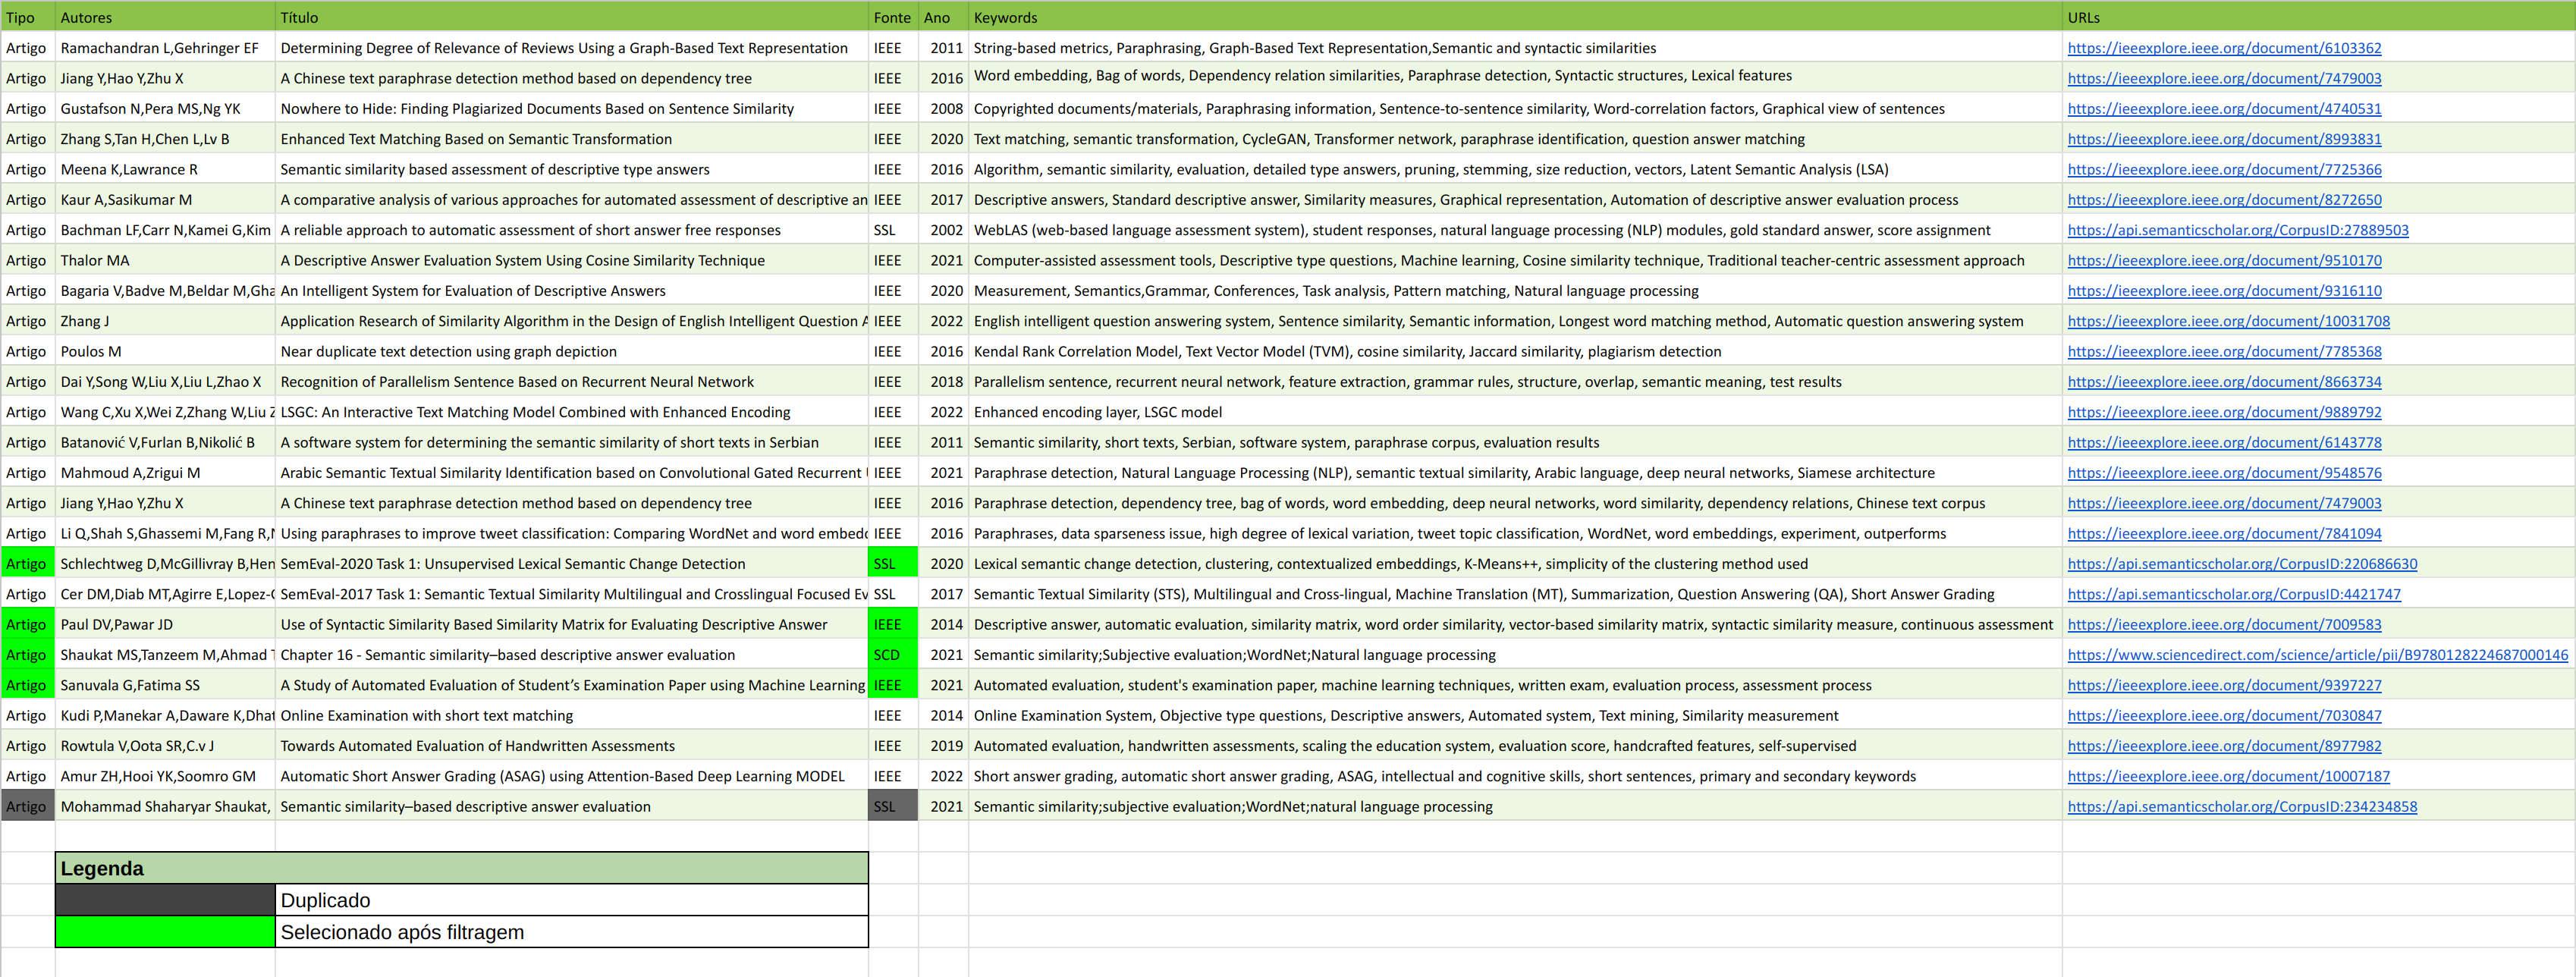
\includegraphics[width=\textwidth]{imgs/rev.png}
%    \caption{Figura da tabela de revisão bibliográfica sumarizada.}
%    \label{fig:1}
%\end{figure}

Após uma filtragem com base nos resumos e palavras-chaves, tendo como critério, a semelhança dos termos e a similaridade de outros artigos em comparação com a proposta do presente artigo, foram selecionados quatro artigos como base para a revisão bibliográfica como consta na Tabela \ref{table:2}, para leitura integral de seu conteúdo.

\begin{table}[htb!]
\resizebox{\columnwidth}{!}{%
\begin{tabular}{@{}lrrrr@{}}
\toprule
\textbf{Base} &
  \multicolumn{1}{l}{Total encontrados} &
  \multicolumn{1}{l}{Após remoção dos Duplicados} &
  \multicolumn{1}{l}{Após análise do resumo} \\ \midrule 
IEEE             & 21 & 21 & 2 \\
Science Direct   & 1  & 1  & 1 \\
Semantic Scholar & 4  & 3  & 1 \\ \bottomrule
\end{tabular}%
}
\caption{Tabela do funil de leitura.}
\label{table:2}
\end{table}

\newpage

O artigo proposto por \cite{UnsupervisedLexicalSemanticChangeDetection}, faz o uso de \textit{embeddings} de tipo (\textit{type embeddings}) e \textit{embeddings} contextualizados (\textit{token embeddings}) para representar as palavras. Primeiro, é introduzida a distribuição de frequência de sentido (SFD), e a detecção de mudança binária é definida em termos de limiares de frequência. Após isso, a distância de Jensen-Shannon (JSD) entre as distribuições normalizadas de frequência é utilizada para medir a mudança efetuada.
    
No artigo proposto por \cite{SyntacticSimilarityBasedSimilarityMatrixForEvaluatingDescriptiveAnswer}, podemos destacar que o trabalho utiliza a técnica de Análise Semântica Latente (LSA), que é comumente usada para determinar a similaridade de documentos, mas ressalta suas limitações em documentos curtos. O artigo destaca a ausência de abordagens anteriores que se concentrem na avaliação automática de respostas descritivas usando vetores de ordem de palavras. O método proposto utiliza uma matriz de similaridade entre vetores de ordem de palavras para avaliar respostas descritivas. A similaridade entre os vetores é calculada por meio de uma métrica de similaridade sintática, ou seja baseada na ordem das palavras. Os resultados indicam que a abordagem baseada em ordem de palavras é promissora para a avaliação automática de respostas descritivas. A matriz de similaridade é apresentada como uma ferramenta eficaz para computar as notas de cada pergunta.
    
Na proposta do artigo escrito pelos autores \cite{SemanticSimilarityBasedDescriptiveAnswerEvaluation}, pode-se destacar que a pesquisa faz uso de Processamento de Linguagem Natural (NLP) para automatizar o processo de avaliação, especialmente a similaridade de cosseno e índices de similaridade, são empregadas para atribuir notas às respostas.
    
Os autores \cite{StudyAutomatedEvaluationStudentsExaminationPaperMachineLearningTechniques} incorporam uma abordagem que emprega ferramentas de Reconhecimento Óptico de Caracteres (OCR) para extrair texto de respostas manuscritas digitalizadas. A ênfase principal, no entanto, recai sobre o emprego de técnicas avançadas de processamento de linguagem natural para aprimorar a avaliação. O estudo destaca a importância de etapas como a tokenização, remoção de stop words e verificação de sinônimos e antônimos no pré-processamento das respostas. Além disso, aborda a criação de modelos semânticos e o cálculo de similaridade sem mencionar explicitamente as métricas de Machine Learning utilizadas.



No contexto da revisão bibliográfica, alguns conceitos importantes foram retirados dos artigos selecionados, para contribuir com o presente trabalho. Dentre esses, destacam-se a análise da similaridade semântica com cossenos, a consideração da frequência de Sentidos de Palavras (SFD) e a utilização de vetores de ordem de palavras como elementos-chave.

A análise de similaridade semântica com cossenos é uma técnica importante, conforme evidenciado nos artigos revisados \cite{SemanticSimilarityBasedDescriptiveAnswerEvaluation}. Essa abordagem é frequentemente empregada para medir a proximidade semântica entre textos.

O uso da Frequência de Sentidos de Palavras (SFD) em um dos artigos indica a importância específica da distribuição de frequência das palavras. Esse conceito pode contribuir para o trabalho, sendo relevante para aspectos da sintaxe e da semântica do texto.

A utilização de vetores de ordem de palavras, como abordado em um dos artigos, resalta a importância da ordem das palavras na avaliação de respostas descritivas. Essa técnica pode superar limitações associadas à Análise Semântica Latente (LSA) em documentos curtos, oferecendo uma abordagem promissora para a avaliação automática.

Em síntese, a revisão bibliográfica gerou a necessidade de explicitar conceitos fundamentais a análise de similaridade semântica com cossenos, a distribuição de frequência de sentidos de palavras e da exploração de vetores de ordem de palavras como pontos relevantes nos estudos revisados.

\newpage
\chapter{Metodologia}

\section{Abordagem de pesquisa:}
Levando em conta que o presente trabalho possui como objetivo realizar avaliação automática de respostas dissertativas, pretende-se que o resultado final do mesmo seja uma proposta de resolução desse problema. Assim, podemos classificar sua abordagem de metodologia como experimental, haja vista que serão realizados experimentos com os dados e as técnicas, que serão descritas no decorrer do texto, afim de atingir o objetivo proposto.

%O presente trabalho possui a abordagem exploratória, haja vista que, desejamos avaliar o desempenho de diferentes técnicas de NLP para avaliação de um grau de parafraseamento entre as respostas. Afim de obter uma clareza maior em que técnicas podem ter um melhor desempenho no trabalho de avaliar questões dissertativas. 

%Em relação ao método, podemos encaixar o estudo como um estudo de corte, pois serão analisados quais parâmetros contidos nos textos podem influenciar na similaridade semântica de seu conteúdo com o texto de referência. Também podemos relacionar nosso estudo com estudos de caso, já que alguns dos dados utilizados serão específicos de exames realizados no Centro Universitário FEI, o que gerará uma compreensão de quais variáveis influenciaram o resultado e detalhes específicos do caso que podem ser relevantes para o caso.

\section{Bases de dados:}
Como fonte principal de dados, utilizaremos o \textit{DataSet ASQA (Answer Summaries for Questions which are Ambiguous)} da \textit{Google Research} em parceria com as universidade de \textit{Duke University} e \textit{Cornell University}, o \textit{DataSet} contém respostas dissertativas para questões com perguntas ambíguas, isso permitirá a construção dos experimentos e refino das técnicas que serão utilizadas no presente trabalho \cite{dataSetGoogleASQA}.


Além da fonte principal de dados, planejamos também utilizar dados das respostas dissertativas dos alunos de Ciência da Computação do Centro Universitário FEI para questões dissertativas do ENADE.

Ademais, existe a possibilidade de que um futuro questionário seja confeccionado para que, com a ajuda voluntária dos alunos da mesma instituição, mais dados sejam coletados e usados no presente trabalho. Essa possibilidade será investigada caso seja necessário.

%Faremos uso de uma base de dados própria fornecida pela Professora Leila Bergamasco, a base contém as respostas dissertativas das questões de um simulado do ENADE, constam apenas respostas de alunos do Centro Universitário FEI, integrantes do curso de Ciência da Computação entre o 5° e 8° ciclo. Ademais, 

\section{Materiais:}
Serão utilizados computadores para o desenvolvimento da experimentação e a documentação do processo. Os computadores principais utilizados serão de posse própria, caso seja necessário, também podem ser utilizados computadores disponibilizados no campus do Centro Universitário FEI. 

Se no decorrer do processo de experimentação, dificuldades em relação as capacidades de processamento e memórias dos computadores forem identificados, abre-se também a possibilidade do uso de plataformas disponibilizadas \textit{online}, como o \textit{Google Colab} (\url{https://colab.google/}) e a \textit{Weights \& Biases} (\url{https://wandb.ai/site/}), ambas oferecem possibilidade de uso gratuito para estudantes que utilizarem apenas com fins acadêmicos.

\section{Métodos:}
Serão utilizados métodos de NLP, tais como mineração de texto, medição de distância de cossenos (para mensurar similaridade de textos), frequência de sentidos de palavras (SFD), presença de palavras-chaves (KW), ordem de sequência das palavras, entre outros. Para compor toda a metodologia, pretende-se elaborar uma métrica de avaliação do grau de similaridade semântica entre dois conteúdos. 

Assumindo que dois textos possuem exatamento o mesmo conteúdo, sua similaridade poderia ser descrita em uma escala percentual como 100\%, por outro lado, haverão textos que possuirão conteúdo sintaticamente diferentes, logo, espera-se que seu percentual de similaridade diminua, porém, ainda assim seria possivel a existência de similaridade semântica entre esse texto e a respota correta, sendo assim, é importante avaliar aspectos semânticos do texto. 

Desta forma, a hipótese é que, para avaliarmos tal similaridade, será necessário avaliar uma série de fatores importantes que irão compor a métrica de avaliação proposta. Esses fatores seriam:
\begin{itemize}
    \item \textbf{As propriedades da sintaxe do texto:} Tal fator será levado em consideração tendo em vista que os trabalhos avaliados na revisão bibliográfica demonstraram a importância de propriedades sintáticas como a ordem em que as sequências de palavras estão posicionadas no texto.
    \item \textbf{Frequência de Sentidos de Palavras (SFD):} Pois também foi demonstrado nos trabalhos avaliados na revisão bibliográfica que essa medida estatística é relevante para a avaliação das respostas.
    \item \textbf{A medição da distância de cossenos:} Essa medida tem relevância para a métrica pois mensura a similaridade semântica entre dois textos através de suas representações vetoriais.
    \item \textbf{A presença de palavras-chave (\textit{keywords}):} Serão palavras definidas para cada questão pelo seu confeccionador como termos com um grau mais elevado de relevância para a resposta esperada do aluno. determinadas como parte da resposta padrão para aquela questão.
\end{itemize}

Todos os fatores apresentados acima já foram utilizados de maneira isolada por diferentes trabalhos como uma forma de avaliação. No caso do presente trabalho pretende-se realizar uma junção dos fatores em uma métrica única para avaliação, averiguando-se ao longo do desenvolvimento do trabalho qual a relevância de cada um deles, para que um peso ajustado seja atribuído para cada fator da métrica. 

Caso a métrica proposta acima apresente bons resultados, pode-se cogitar a elaboração de uma segunda métrica, em que dois outros fatores seriam adicionados como uma possível melhoria à primeira, sendo eles: 
\begin{itemize}
    \item A verificação da possibilidade de um texto ser classificado como paráfrase de outro, já que o trabalho possui como hipótese que toda resposta correta é em algum grau uma paráfrase da resposta modelo. Com a identificação da paráfrase, como pode ser feita a medição do grau de parafraseamento entre os dois textos.
    \item A quantidade de modificações necessárias para que a resposta fornecida seja transformada lexicalmente e sintaticamente na resposta modelo.
\end{itemize}
Esses dois fatores não foram considerados nos trabalhos revisados anteriormente, na eventual proposta de uma segunda métrica, ter-se-á como hipótese que os dois fatores resultarão em uma melhoria no resultado.

A proposta da métrica pode ser matemáticamente descrita como na Equação 2, que contém a equação de uma média ponderada.
\begin{equation}
Métrica1 = \frac{fator1 \times peso_{1} + fator2 \times peso_{2} + fator3 \times peso_{3} + fator4 \times peso_{4}}{\sum_{i=1}^{4}peso_{i}}
\end{equation}

Em que \textit{fator1} são as propriedades sintáticas do texto, o \textit{fator2} representa o SFD, o \textit{fator3} é a distância de cossenos e o \textit{fator4} é referente as \textit{keywords}. 

Como resultado a métrica deverá fornecer um número no intervalo de 0  100 que, quanto maior, indica maior proximidade semântica entre os textos e uma maior probabilidade de acerto da resposta fornecida por um aluno. 

No caso da segunda métrica, o diferencial seria adição dos dois outros fatores para mensurar o grau de parafraseamento e a quantidade de modificações, sendo respectivamente o \textit{fator5} e o \textit{fator6} como descrito na Equação 3.

\begin{equation}
\tiny Métrica2 = \frac{fator1 \times peso_{1} + fator2 \times peso_{2} + fator3 \times peso_{3} + fator4 \times peso_{4} + fator5 \times peso_{5} + fator6 \times peso_{6}}{\sum_{i=1}^{6}peso_{i}}
\end{equation}

\section{Avaliação:}
Para avaliação do desempenho das técnicas propostas, as bases de dados serão divididas em duas, uma primeiramente para treinamento e refino dos experimentos. Após os resultados estarem satisfatórios, a segunda parte dos dados será utilizada para a validação dos resultados obtidos pelo algoritmo, verificando se estão condizente com os resultados fornecidos pelas avaliações registradas nos dados e se seu funcionamento é geral ou se há algum viés nos resultados. Uma representação visual das etapas gerais imaginadas para o processo pode ser vista na Figura \ref{figure:4}.

\begin{figure}[h!]
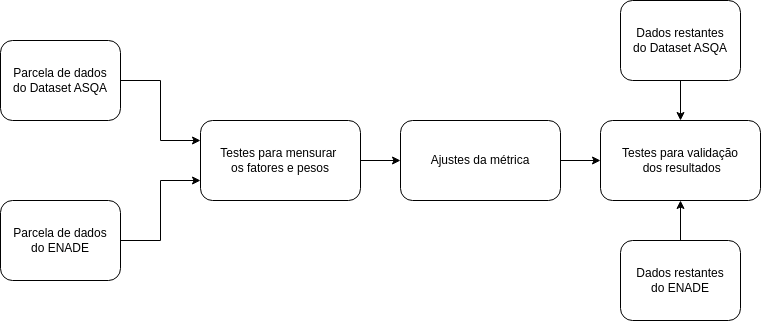
\includegraphics[width=\textwidth]{./imgs/diagramasTcc.png}
\caption{Diagrama geral das etapas do processo.}\label{figure:4}
\end{figure}

% olhar depois:

% https://www.researchgate.net/publication/337412528_Avaliacao_Automatica_de_respostas_discursivas_curtas_baseado_em_tres_dimensoes_linguisticas

% https://revistas.unoeste.br/index.php/ce/article/view/4595

% https://physionet.org/content/radqa/1.0.0/

% https://ppgee.propesp.ufpa.br/ARQUIVOS/teses/tese_abntex_final.pdf

% dataset search google

\newpage
\chapter{PROPOSTA EXPERIMENTAL}

Como proposta experimental, será realizado a avalição das questões dissertativas através de um algoritmo que leva em consideração a métrica de pontuação proposta nos capitulos anteriores do texto, tanto com seus fatores em conjunto, quanto com eles individualmente, o resultado das avaliações realizadas pelo algoritmo será comparado aos valores de avaliação dos professores que estão presentes nas bases de dados específicadas anteriormente no capítulo de metodologia.

A proposta experimental pode ser dividida nos seguintes tópicos:
\begin{itemize}
	\item \textbf{Avaliação individual da presença de palavras chaves:} O algoritmo proposto deve avaliar se as palavras chaves determinadas para aquela questão, estão presentes no texto e pontuar com base na quantidade de palavras-chave encontradas. Tendo como hipótese que essa avaliação individualemte não fornecerá um resultado com alta precisão.
	\item \textbf{Avalição individual da frequência de palavras (SFD):} O algoritmo realizará a medição da frequência das palavras no texto da resposta padrão e da resposta fornecida pelo aluno, cada palavra terá sua frequência em ambos os textos e a diferença entre as duas será medida em porcentagem. Caso palavras diferentes apareçam no texto da respota do aluno, podemos levar em consideração inicialmente a possibilidade de descartá-las, outras possibilidades futuras também podem ser consideradas caso melhores abordagens sejam encontradas na literatura científica.
	\item \textbf{Avalição individual da sintaxe do texto:} Utilizando vetores de ordem de palavras o algoritmo deve realizar a medição das métricas de sintaxe do texto, primeiramente da resposta padrão, em sequência, das respotas dos alunos. O vetor de ordem de palavras da respota padrão será comparado com os vetores de ordem de palavras que representem as respostas dos alunos.
	\item \textbf{Avaliçao semantica através da distância de cossenos:} Na avaliação da distância de cossenos  os textos serão representados em vetores de palavras que representam a similaridade direcional, não a ordem como no item anterior, conforme os ângulos calculado entre os vetores diminui, sabemos que o grau de similaridade entre os textos aumenta. Dentro de diferentes técnicas de medição, a revisão bibliográfica demonstrou que essa é a mais precisa \cite{SemanticSimilarityBasedDescriptiveAnswerEvaluation}.
\end{itemize}

Além das avaliações individuais definidas acima, também serão avaliados os fatores em diferentes conjuntos para que os resultado obtidos através dessas combinções sejam comparados com a junção de todos os quatro fatores em uma só métrica, tendo como hipótese que as métricas com um conjunto de fatores combinados funcionarão melhor do que um fator individualmente e que a métrica de todos os fatores juntos terá o melhor resultado. 

Em todas as métricas combinadas, os diferentes fatores devem possuir pesos que representem o quão relevante cada elemento é para uma avalição da resposta. Com base nas avaliações individuais realizadas inicialmente, serão obtido quais dos fatores possuem uma proximidade maior com os valores das avalições dos professores disponíveis nas bases de dados, podemos, inicialmente, propor que quanto maior a proximidade dos valores individuais obtidos com as avaliações nas bases de dados, mais relevantes esse fator deve ser em seu peso. 

Com o objetivo de obter a melhor precisão possível, os pesos inicias serão modificados para valores com maior ou menor relevância, afim de que o resultado final obtido seja o mais próximo possível dos resultados das avaliações feitas pelos professores disponíveis nas bases de dados. Além disso, métricas como BLEU e ROUGE podem ser empregadas para avaliar a qualidade da pontuação em termos de sobreposição de palavras entre as respostas.

A proposta experimental busca não apenas avaliar a viabilidade do algoritmo, mas também otimizar sua precisão por meio da ponderação adequada dos fatores. A abordagem modular, combinada com a análise iterativa dos pesos, visa criar um sistema capaz de fornecer resultados de avaliação de respostas dissertativas com alta concordância em relação às avaliações humanas.

\section{Cronograma}
Na Tabela \ref{table:3} está estruturado o cronograma proposta para as fases que já concluídas e as que deverão ser concluídas afim de alcaçar os objetivos propostos.

\newcommand{\gray}{\cellcolor{black!25}}
\begin{table}[ht]
\label{tab:cronograma}
\resizebox{\textwidth}{!}{
\begin{tabular}{llllrll|llllll}
\hline
\multicolumn{1}{c}{ } &
  \multicolumn{6}{c|}{2023} &
  \multicolumn{6}{c}{2024} \\ \hline
\multicolumn{1}{|l|}{Atividade / Mês} &
  \multicolumn{1}{l|}{07} &
  \multicolumn{1}{l|}{08} &
  \multicolumn{1}{l|}{09} &
  \multicolumn{1}{r|}{10} &
  \multicolumn{1}{l|}{11} &
  12 &
  \multicolumn{1}{l|}{01} &
  \multicolumn{1}{l|}{02} &
  \multicolumn{1}{l|}{03} &
  \multicolumn{1}{l|}{04} &
  \multicolumn{1}{l|}{05} &
  \multicolumn{1}{l|}{06} \\ \hline
\multicolumn{1}{|l|}{Definição do tema e orientador} &
  \multicolumn{1}{l|}{\cellcolor[HTML]{656565}} &
  \multicolumn{1}{l|}{\cellcolor[HTML]{656565}} &
  \multicolumn{1}{l|}{} &
  \multicolumn{1}{r|}{} &
  \multicolumn{1}{l|}{} &
   &
  \multicolumn{1}{l|}{{\ul }} &
  \multicolumn{1}{l|}{} &
  \multicolumn{1}{l|}{} &
  \multicolumn{1}{l|}{} &
  \multicolumn{1}{l|}{} &
  \multicolumn{1}{l|}{} \\ \hline
\multicolumn{1}{|l|}{Revisão bibliográfica} &
  \multicolumn{1}{l|}{} &
  \multicolumn{1}{l|}{} &
  \multicolumn{1}{l|}{\cellcolor[HTML]{656565}} &
  \multicolumn{1}{l|}{\cellcolor[HTML]{656565}} &
  \multicolumn{1}{l|}{} &
   &
  \multicolumn{1}{l|}{{\ul }} &
  \multicolumn{1}{l|}{} &
  \multicolumn{1}{l|}{} &
  \multicolumn{1}{l|}{} &
  \multicolumn{1}{l|}{} &
  \multicolumn{1}{l|}{} \\ \hline
\multicolumn{1}{|l|}{Planejamento da metodologia} &
  \multicolumn{1}{l|}{} &
  \multicolumn{1}{l|}{} &
  \multicolumn{1}{l|}{} &
  \multicolumn{1}{l|}{\cellcolor[HTML]{656565}} &
  \multicolumn{1}{l|}{\cellcolor[HTML]{656565}} &
   &
  \multicolumn{1}{l|}{{\ul }} &
  \multicolumn{1}{l|}{} &
  \multicolumn{1}{l|}{} &
  \multicolumn{1}{l|}{} &
  \multicolumn{1}{l|}{} &
  \multicolumn{1}{l|}{} \\ \hline
\multicolumn{1}{|l|}{Finalização do relatório parcial} &
  \multicolumn{1}{l|}{} &
  \multicolumn{1}{l|}{} &
  \multicolumn{1}{l|}{} &
  \multicolumn{1}{r|}{} &
  \multicolumn{1}{l|}{} &
  \cellcolor[HTML]{656565} &
  \multicolumn{1}{l|}{{\ul }} &
  \multicolumn{1}{l|}{} &
  \multicolumn{1}{l|}{} &
  \multicolumn{1}{l|}{} &
  \multicolumn{1}{l|}{} &
  \multicolumn{1}{l|}{} \\ \hline
\multicolumn{1}{|l|}{Aprofundamento nos conceitos de NLP} &
  \multicolumn{1}{l|}{} &
  \multicolumn{1}{l|}{} &
  \multicolumn{1}{l|}{} &
  \multicolumn{1}{r|}{} &
  \multicolumn{1}{l|}{} &
   &
  \multicolumn{1}{l|}{\cellcolor[HTML]{656565}{\ul }} &
  \multicolumn{1}{l|}{} &
  \multicolumn{1}{l|}{} &
  \multicolumn{1}{l|}{} &
  \multicolumn{1}{l|}{} &
  \multicolumn{1}{l|}{} \\ \hline
\multicolumn{1}{|l|}{\begin{tabular}[c]{@{}l@{}}Experimentação do algoritmo para\\ avaliação da relevância dos fatores\end{tabular}} &
  \multicolumn{1}{l|}{} &
  \multicolumn{1}{l|}{} &
  \multicolumn{1}{l|}{} &
  \multicolumn{1}{r|}{} &
  \multicolumn{1}{l|}{} &
   &
  \multicolumn{1}{l|}{{\ul }} &
  \multicolumn{1}{l|}{\cellcolor[HTML]{656565}} &
  \multicolumn{1}{l|}{} &
  \multicolumn{1}{l|}{} &
  \multicolumn{1}{l|}{} &
  \multicolumn{1}{l|}{} \\ \hline
\multicolumn{1}{|l|}{\begin{tabular}[c]{@{}l@{}}Experimentação para aprimoramento\\ dos valores dos pesos na métrica\end{tabular}} &
  \multicolumn{1}{l|}{} &
  \multicolumn{1}{l|}{} &
  \multicolumn{1}{l|}{} &
  \multicolumn{1}{r|}{} &
  \multicolumn{1}{l|}{} &
   &
  \multicolumn{1}{l|}{{\ul }} &
  \multicolumn{1}{l|}{} &
  \multicolumn{1}{l|}{\cellcolor[HTML]{656565}} &
  \multicolumn{1}{l|}{} &
  \multicolumn{1}{l|}{} &
  \multicolumn{1}{l|}{} \\ \hline
\multicolumn{1}{|l|}{\begin{tabular}[c]{@{}l@{}}Validação dos resultados obtidos com\\ os dados de avaliações de professores\end{tabular}} &
  \multicolumn{1}{l|}{} &
  \multicolumn{1}{l|}{} &
  \multicolumn{1}{l|}{} &
  \multicolumn{1}{r|}{} &
  \multicolumn{1}{l|}{} &
   &
  \multicolumn{1}{l|}{{\ul }} &
  \multicolumn{1}{l|}{} &
  \multicolumn{1}{l|}{} &
  \multicolumn{1}{l|}{\cellcolor[HTML]{656565}} &
  \multicolumn{1}{l|}{} &
  \multicolumn{1}{l|}{} \\ \hline
\multicolumn{1}{|l|}{\begin{tabular}[c]{@{}l@{}}Adição dos fatores de parafraseamento\\ para implementar a segunda métrica\end{tabular}} &
  \multicolumn{1}{l|}{} &
  \multicolumn{1}{l|}{} &
  \multicolumn{1}{l|}{} &
  \multicolumn{1}{r|}{} &
  \multicolumn{1}{l|}{} &
   &
  \multicolumn{1}{l|}{{\ul }} &
  \multicolumn{1}{l|}{} &
  \multicolumn{1}{l|}{} &
  \multicolumn{1}{l|}{} &
  \multicolumn{1}{l|}{\cellcolor[HTML]{656565}} &
  \multicolumn{1}{l|}{} \\ \hline
\multicolumn{1}{|l|}{\begin{tabular}[c]{@{}l@{}}Ajustes finais para refinamento do \\ algoritmo e finalização do projeto \\ (Relatório final e material do INOVA FEI)\end{tabular}} &
  \multicolumn{1}{l|}{} &
  \multicolumn{1}{l|}{} &
  \multicolumn{1}{l|}{} &
  \multicolumn{1}{r|}{} &
  \multicolumn{1}{l|}{} &
   &
  \multicolumn{1}{l|}{{\ul }} &
  \multicolumn{1}{l|}{} &
  \multicolumn{1}{l|}{} &
  \multicolumn{1}{l|}{} &
  \multicolumn{1}{l|}{} &
  \multicolumn{1}{l|}{\cellcolor[HTML]{656565}} \\ \hline
\end{tabular}
}
\caption{Cronograma de execução do projeto}
\label{table:3}
\end{table}

\newpage
\chapter{CONCLUSÃO}
Levando em consideração tudo o que foi exposto ao longo de todos os capítulos, pode-se concluir, deste trabalho, que propôs uma abordagem para automatizar o processo de avaliação de respostas dissertativas, que os resultados obtidos apontam para uma direção interessante e promissora. Foi possível gerar uma grande quantidade de avaliações com resultados próximos aos de avaliações de professores. A métrica proposta, que levou em consideração a frequência de termos, distância de Levenshtein e similaridade semântica obtidas através de modelos BERT, visando simplificar o processo de correção manual para possibilitar a análise do desempenho dos alunos mais rapidamente, demonstrou seu funcionamento com resultados razoáveis e compreensíveis dentro dos limites do que este trabalho teve como proposta. Ao utilizar os \textit{DataSets} de diferentes temáticas e idiomas, foi possível estimar pesos para os fatores que compõem a métrica de avaliação. Com eles, gerar avaliações automáticas e coletar os dados de acurácia da métrica, que apresentaram um resultado que pode ser considerado satisfatório para os fatores presentes e a quantidade de dados disponibilizados, além do tempo disponível para conclusão deste trabalho.

Algumas limitações foram observadas nos resultados, em que no caso de alguns \textit{datasets}, foi possível ver uma quantidade grande de erros em faixas percentuais muito altas. Avaliações com uma diferença de valor alta quando comparadas com as avaliações dos professores. Uma explicação para muitos desses casos é a falta de compreensão de mais fatores relativos ao texto que o algoritmo ainda não possui a capacidade de avaliar.

Tendo isso em vista, como possibilidades de trabalhos futuros para melhoria dos resultados, algumas abordagens podem ser consideradas, como por exemplo:

\begin{itemize}
    \item \textbf{Inclusão de mais fatores no algoritmo}: Avaliar a inclusão de mais fatores ou características no algoritmo pode ajudar a capturar melhor a complexidade das respostas dissertativas em diferentes idiomas. Fatores como identificação de paráfrases e mais características da semântica do texto podem ajudar a alcançar uma métrica mais acertiva.
    \item \textbf{Uso de outros modelos ou redes neurais}: Comparar o desempenho do algoritmo de regressão linear com outros modelos ou redes neurais pode fornecer boas considerações sobre qual abordagem é mais eficaz para determinação dos pesos.
\end{itemize}

Essas abordagens podem ajudar a aprimorar a precisão e a generalização do algoritmo para qualquer temática, tornando-o mais robusto e eficaz na avaliação de respostas dissertativas em português, inglês, espanhol ou até outros idiomas, eventualmente.

Em relação às questões de pesquisa levantadas para este trabalho, podemos considerar que:

\begin{enumerate}
    \item Os parâmetros extraídos foram capazes de avaliar uma grande quantidade de respostas, embora com a complementação de mais fatores e mais dados para treinamento com outros modelos, os resultados podem ser melhorados.
    \item Esses parâmetros foram capazes de definir uma pontuação que funcionou de maneira geral para avaliação de respostas dissertativas, embora houvessem limitações na acurácia da métrica.
    \item Os fatores devem ser ponderados com pesos, que podem ser otimizados com um volume maior de dados ou outros algoritmos de inteligência artificial, como redes neurais, para determiná-los.
    \item Podemos constatar que a acurácia da métrica variou consideravelmente comparando os idiomas e também o volume de dados para treinamento e teste. Isso fez com que os valores de acurácia do algoritmo fossem mais próximos quando treinados com os \textit{datasets} em inglês e espanhol.
\end{enumerate}

Em última análise, este trabalho almejou não apenas uma solução para as limitações atuais na avaliação de respostas dissertativas, mas também contribuir para a determinação de quais parâmetros são relevantes em uma métrica para esse problema de pesquisa. Com a determinação mais detalhada e profunda desses parâmetros em trabalhos futuros, abre-se a possibilidade do surgimento de uma contribuição significativa para os processos educacionais, proporcionando aos professores uma ferramenta valiosa para avaliação e acompanhamento do progresso dos alunos.

\printbibliography

\end{document}
